\documentclass[10pt,executivepaper]{article}
\usepackage[utf8]{inputenc}
\usepackage[spanish]{babel}
\usepackage{amsmath}
\usepackage{amsfonts}
\usepackage{amssymb}
\usepackage{graphics}
\usepackage{graphicx}
\usepackage[left=2cm,right=2cm,top=2cm,bottom=2cm]{geometry}
\usepackage{imakeidx}
\makeindex[columns=3, title=Alphabetical Index, intoc]
\usepackage{listings}
\usepackage{xcolor}
\usepackage{multicol}
\usepackage{changepage}
\usepackage{float}
\usepackage{cite}
\usepackage{url}
\usepackage{pdflscape}

\definecolor{codegreen}{rgb}{0,0.6,0}
\definecolor{codegray}{rgb}{0.5,0.5,0.5}
\definecolor{codepurple}{rgb}{0.58,0,0.82}
\definecolor{backcolour}{rgb}{0.95,0.95,0.92}

\lstdefinestyle{mystyle}{
    backgroundcolor=\color{backcolour},
    commentstyle=\color{codegreen},
    keywordstyle=\color{magenta},
    numberstyle=\tiny\color{codegray},
    stringstyle=\color{codepurple},
    basicstyle=\ttfamily\footnotesize,
    breakatwhitespace=false,
    breaklines=true,
    captionpos=b,
    keepspaces=true,
    numbers=left,
    numbersep=5pt,
    showspaces=false,
    showstringspaces=false,
    showtabs=false,
    tabsize=3
}

\def\fillandplacepagenumber{%
 \par\pagestyle{empty}%
 \vbox to 0pt{\vss}\vfill
 \vbox to 0pt{\baselineskip0pt
   \hbox to\linewidth{\hss}%
   \baselineskip\footskip
   \hbox to\linewidth{%
     \hfil\thepage\hfil}\vss}}


\lstset{style=mystyle}

\title{Actividad: Chat multicast}

\author{Instituto Politécnico Nacional\\Escuela Superior de Computo\\Desarrollo de Sistemas Distribuidos\\Adrian González Pardo\\4CV1\\21/01}
\date{\today}
\newcommand\tab[1][1cm]{\hspace*{#1}}

\begin{document}
% Portada
%encabezado
\begin{minipage}{0.4\textwidth}
	\begin{flushleft}
		
\includegraphics[scale = 0.05]{logoescom.png}
	\end{flushleft}
\end{minipage}
\begin{minipage}{0.51\textwidth}
	\begin{flushright}
		
\includegraphics[scale = 0.055]{logoipn.png}
	\end{flushright}
\end{minipage}
\begin{center}
	\par\vspace{0.5cm}{
	\huge\textbf{Instituto Politécnico Nacional \\*[0.20cm] Escuela Superior de Cómputo}}
\par\vspace{1cm}{
	\large\textbf{Desarrollo de Sistemas Distribuidos\\Actividad: Chat Multicast\\Curso impartido por el profesor: Pineda Guerrero Carlos\\Grupo: 4CV1\\21/01\\Alumno: Adrian González Pardo\\}
}
\par\vspace{1cm}{
	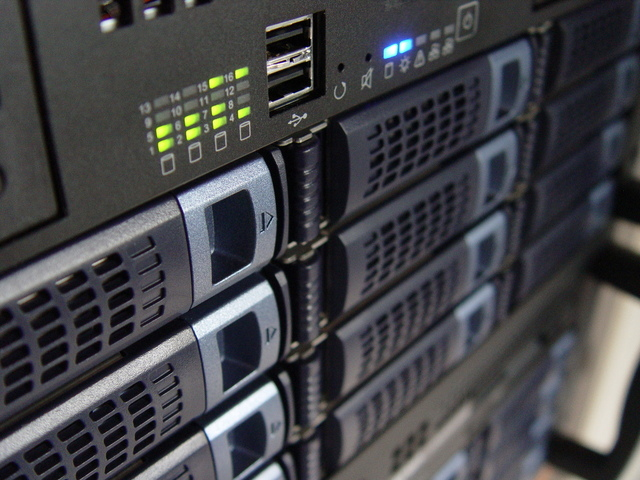
\includegraphics[scale=0.5]{servers.jpg}
}
\par\vspace{2cm}{
	Ultima fecha modificado: \today
}
\end{center}

% Indice
\clearpage
\section{Desarrollo}
Para el desarrollo necesario de esta practica es necesario realizar el uso de paquetes nativos de java los cuales son el uso Sockets, Buffer de lectura de datos, Entrada de datos por teclado, Hilos, y algunas otras cosas más que vienen en el código fuente. por ello se programo un chat de multicast el cual debido a que no conocemos el tamaño de datos de entrada, haremos uso de una restricción que viene en nuestra tarjeta de red en Linux, el cual es un maximo de datos de 1500 por ello en caso de que sobren datos el mismo programa enviara los datos de forma serializada y un poco instantanea.
\section{Código fuente:}
\begin{center}
  \lstinputlisting[language=Java]{../Chat.java}
  \lstinputlisting[language=Bash]{../Makefile}
\end{center}
\section{Ejecución en red}
\textbf{Para este caso se realizo una implementación a nivel red Local con al menos 4 equipos, se puede hacer lo siguiente (destacando que ya hay un emparejamiento de llaves ssh) y ellos mismos se uniran al grupo de Multicast}\\
A nivel local se conoce la lista de los siguientes equipos:
\begin{itemize}
  \item Lenovo IP: 192.168.100.69
  \item Acer IP: 192.168.100.3
  \item Raspberry Pi 3B IP: 192.168.100.194
  \item Raspberry Pi 4B IP: 192.168.100.103
\end{itemize}
Para el cual se envio los datos con el siguiente script:
\begin{center}
  \lstinputlisting[language=Bash]{../script.sh}
\end{center}

\section{Capturas y descripción del programa}
\begin{center}
  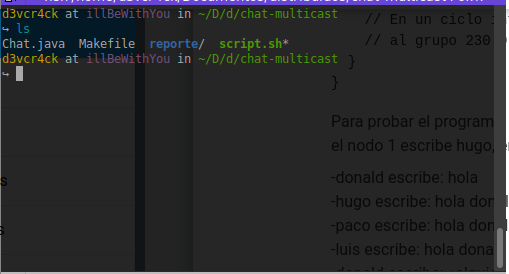
\includegraphics[scale=0.5]{img/antes.png}
  \\\textit{Figura 1: Antes de la compilación con Makefile}
  \\
  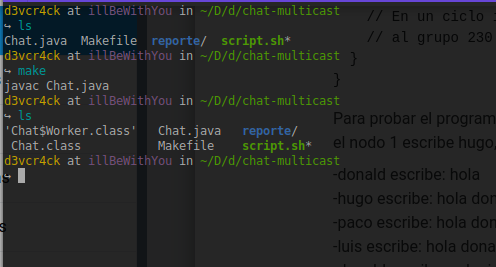
\includegraphics[scale=0.5]{img/compilacion.png}
  \\\textit{Figura 2: Compilación}
  \begin{landscape}
    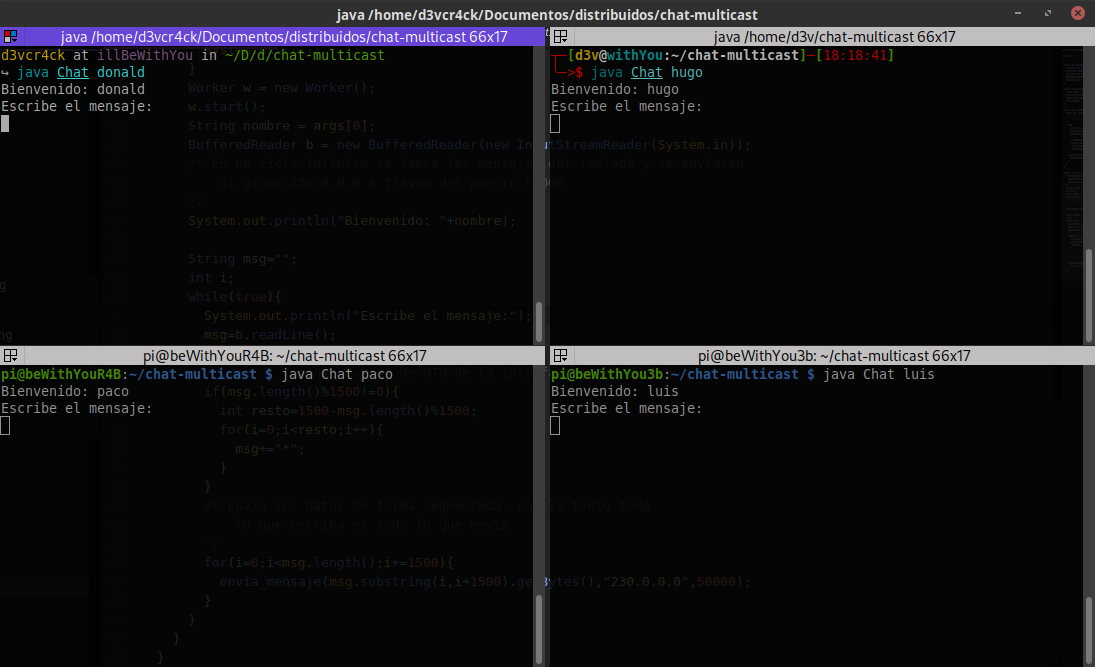
\includegraphics[scale=0.5]{img/prompt.png}
    \\\textit{Figura 3: Prompt del chat de multicast.}
    \fillandplacepagenumber

    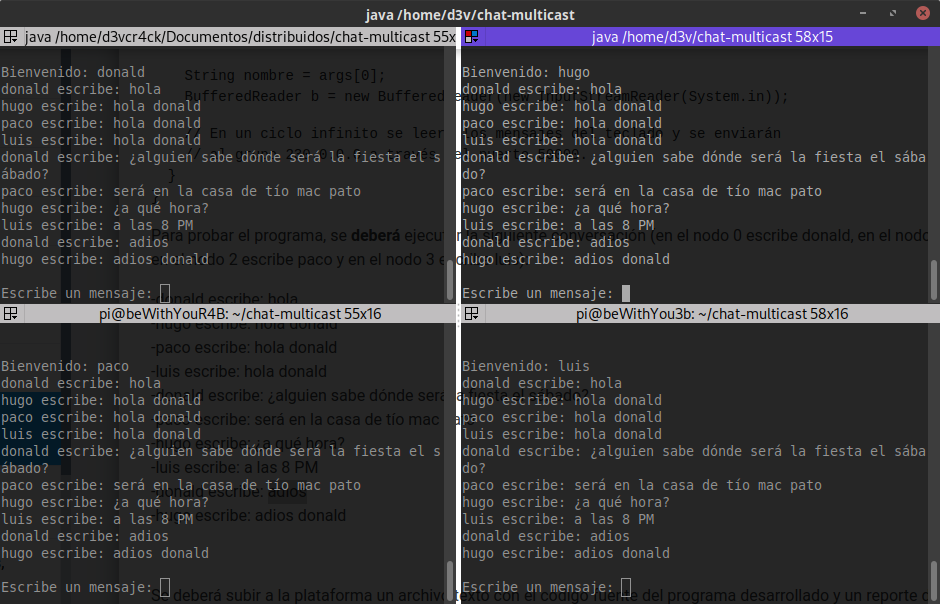
\includegraphics[scale=0.5]{img/terminal-chat.png}
    \\\textit{Figura 4: Ejecución del chat donde llegan los nuevos mensajes.}
    \fillandplacepagenumber
  \end{landscape}
\end{center}

\section{Conclusiones}
El realizar este tipo de programas cuya ejecución se puede realizar de forma universal o en cualquier equipo de cómputo, es gracias a que existe un estandar de red y gracias a la parte de Java de ser un lenguaje multiplataforma el cual nos permite compilar en multiples arquitecturas con diferentes versiones del mismo jdk, por ello es necesario reconocer que igual existen otros lenguajes los cuales nos permiten realizar las mismas tareas.

\end{document}
